
  \section{Results with features from Cesetti et al. (2013)}
\label{app:figures:irtf}


\begin {figure*}
 \centering
  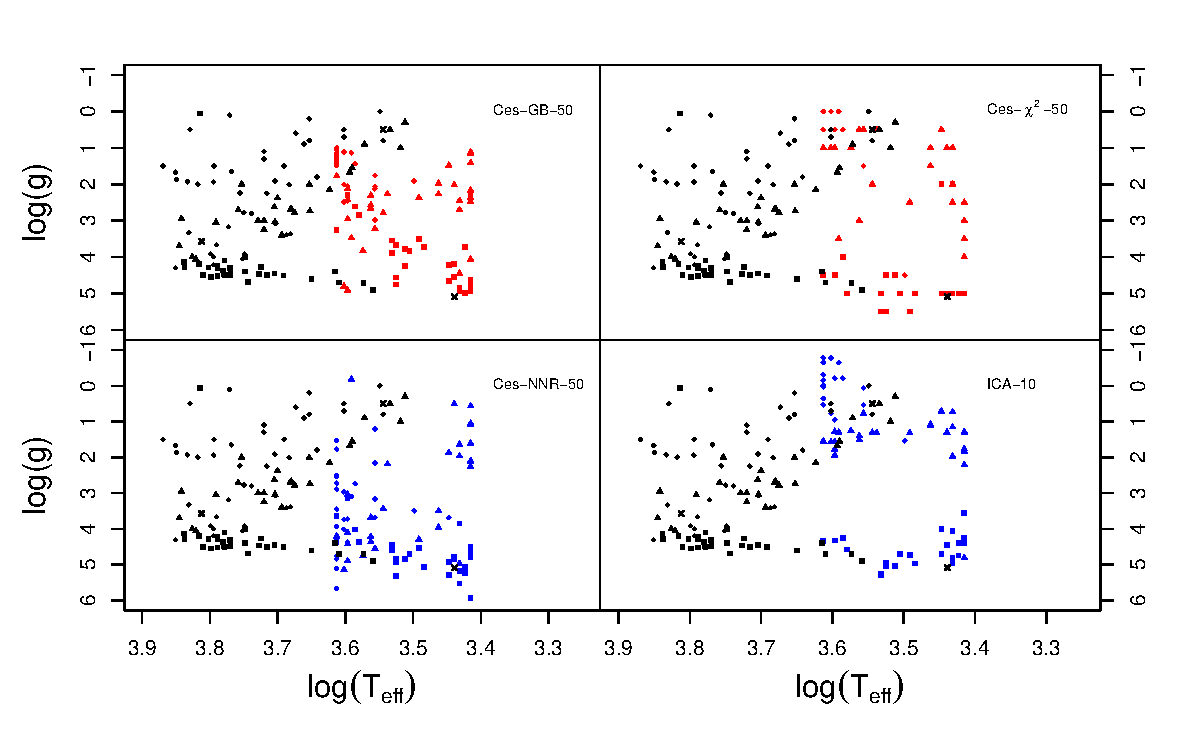
\includegraphics[width=\textwidth]{figs/irtf-figs/irtf-Cesseti}
  \caption{$\log(T_{eff})$--$\log(g)$ diagrams produced by the CES-KNN
    (SNR=$\infty$) effective temperatures, and gravities derived for
    the IRTF collection of spectra with the CES-GB (SNR=50),
    CES-$\chi^2$ (SNR=50), CES-NNR (SNR=50), and $ICA-10$ models
    (clockwise, starting from the top left plot).}
 \label{fig:irtf-ces}
\end {figure*}



\begin {figure}
\centering
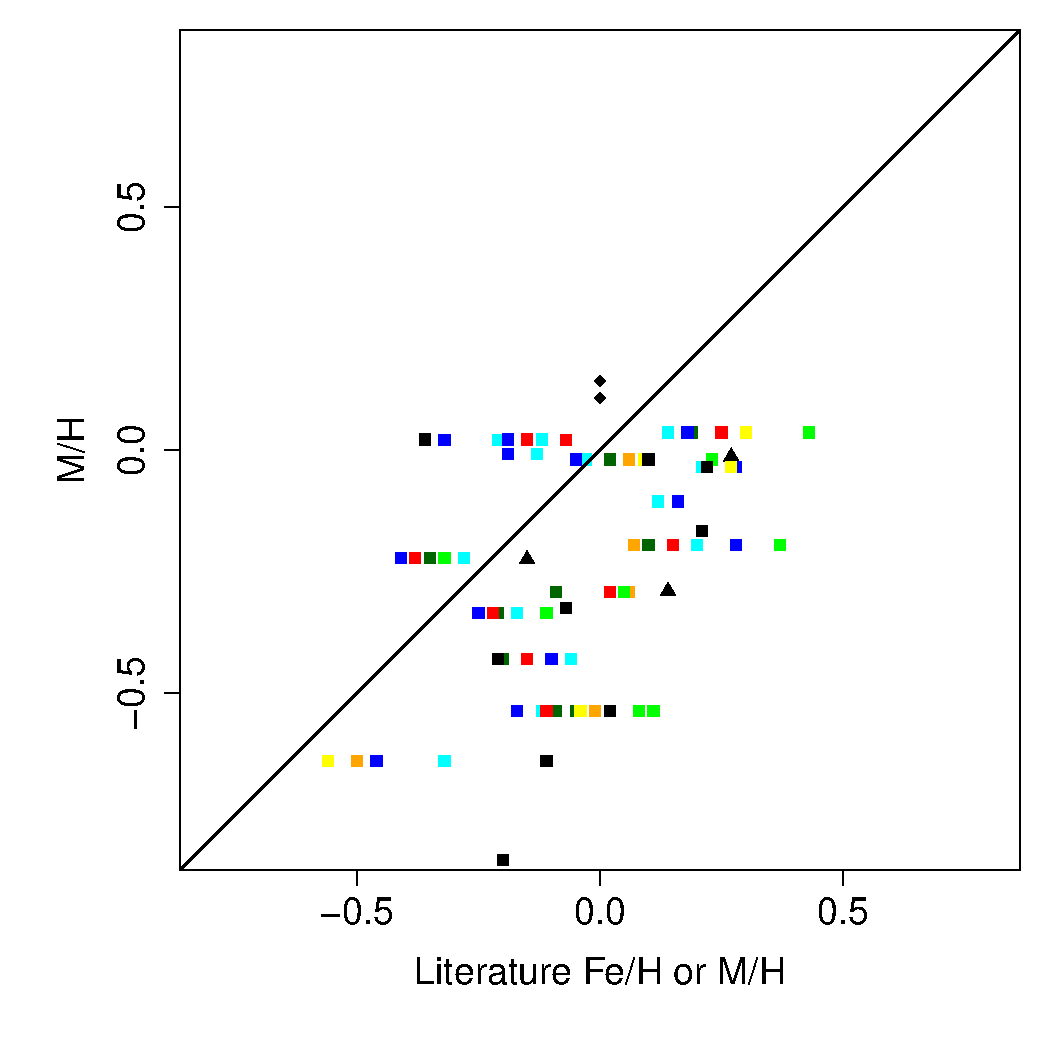
\includegraphics[width=0.45\textwidth]{figs/irtf-figs/M-CES}
\caption{Comparison of the CES-RF (SNR=50) regression model
  predictions for the IRTF collection of spectra with the estimates of
  the metallicity in the literature. The symbols and colours are the
  same as in Figure \ref{MIRTF_ICA_10}.}
\label{fig:irtf-ces-met}
\end {figure}


\begin {figure*}
 \centering
  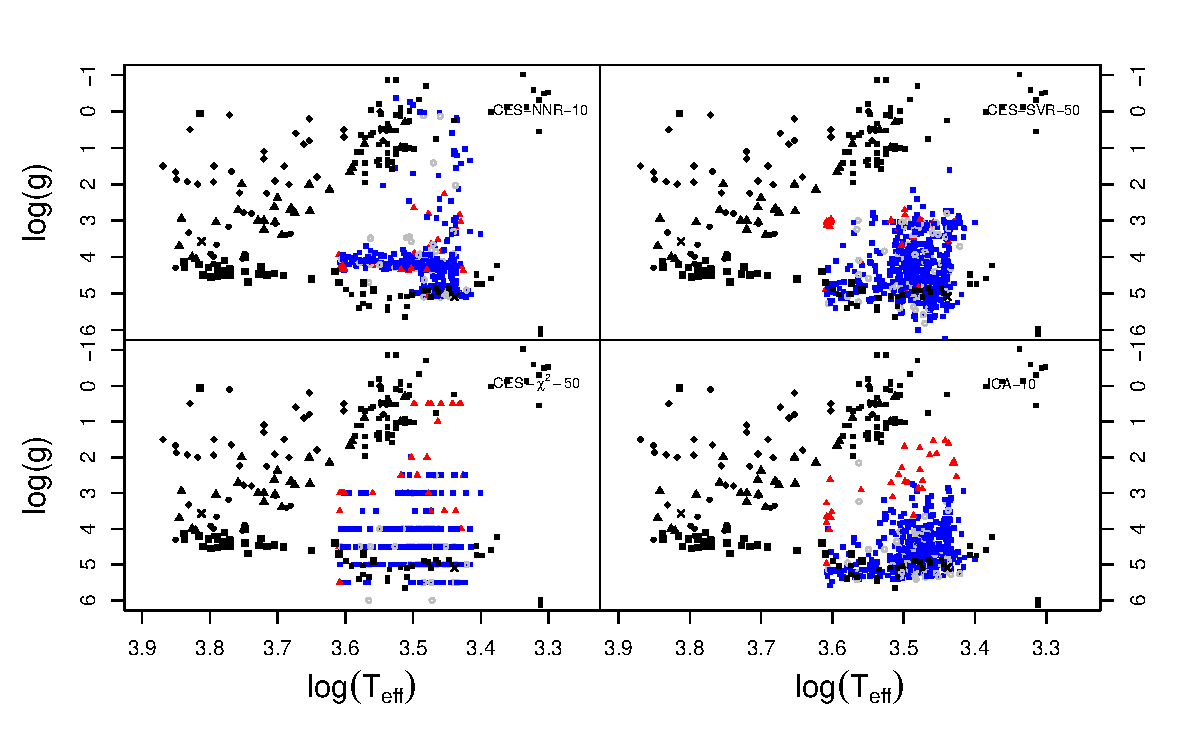
\includegraphics[width=\textwidth]{figs/ipac-Cesseti}
  \caption{$\log(T_{eff})$--$\log(g)$ diagrams produced by the CES-KNN
    (SNR=$\infty$) effective temperatures, and gravities derived for
    the Dwarf Archives collection of spectra with the CES-NNR (SNR=10), CES-SVR
    (SNR=50), CES-$\chi^2$ (SNR=50), and $ICA-10$ models (clockwise,
    starting from the top left plot).}
 \label{fig:ipac-ces}
\end {figure*}



